\chapter{Testowalność oprogramowania}
\label{testowalnosc}
\section{Pojęcie testowalności i~pielęgnowalności \newline oprogramowania}
Termin „testowalność oprogramowania” \footnote{Definicja testowalności według standardu ISO9126}  według definicji ISTQB \footnote{International Software Qualification Board}  i~ISO9126, to właściwość tego oprogramowania umożliwiająca testowanie go po zmianach. Termin ten ściśle powiązany jest także z~innym pojęciem ze słownika testerskiego – pielęgnowalnością. Pielęgnowalność \footnote{Definicja pielęgnowalności według ISTQB}definiowana jest jako łatwość, z~którą oprogramowanie może być modyfikowane w~celu naprawy defektów, dostosowania do nowych wymagań, modyfikowane w~celu ułatwienia przyszłego utrzymania lub dostosowania do zmian zachodzących w~jego środowisku.

\section{Czy testowanie jest potrzebne?}
\label{czy_testowanie_potrzebne}
Po co tak w~ogóle właściwie testować oprogramowanie? Czy testowanie jest potrzebne? Jak dużo testów należy przeprowadzić, aby testowanie było wystarczająco skuteczne? To są pytania, które mogą być tematem osobnej publikacji, w~tym rozdziale poruszone zostaną więc tylko pojęcia, które wykorzystane są w~dalszej części tej pracy.

Człowiek, jako istota żywa i~omylna, może popełnić podczas pracy \textit{błąd}, czyli inaczej – \textit{pomyłkę}. Pomyłka w~pracy programisty może skutkować pojawieniem się \textit{defektu} (usterki, pluskwy) w~kodzie programu, bądź w~dokumentacji. Do tej pory nic się nie dzieje złego, ale jeżeli kod programu, który posiada w~sobie taki defekt, zostanie wykonany, system może nie zrobić tego, co od niego się wymaga, lub wykonać to niezgodnie z~założeniami. Czyli inaczej rzecz ujmując, ulegnie \textit{awarii}. 

Defekty powstają, ponieważ ludzie są omylni, ale pomyłka człowieka, to nie jedyny powód awarii systemów. Mogą one być również spowodowane przez warunki środowiskowe, takie jak promieniowanie, pole magnetyczne i~elektryczne, czy nawet zanieczyszczenia środowiska.

Czy testowanie powoduje całkowite wyeliminowanie awarii systemów? Na pewno nie, ale pozwala je drastycznie ograniczyć. Za pomocą zestawu testów można zmierzyć jakość oprogramowania wyrażoną przez ilość znalezionych usterek oraz budować zaufanie do jakości oprogramowania, jeżeli testerzy znajdują ich mało, bądź nie znajdują ich wcale.

Należy jednak pamiętać, że testowanie samo w~sobie nie poprawia jakości oprogramowania. Dopiero umiejscowienie defektu w~kodzie programu (zdebugowanie) oraz naprawa tego błędu przez programistę poprawi jakość. Tabela \ref{tab:koszty_bledu} przedstawia poglądowo, jak testowanie na poszczególnych etapach wytwarzania oprogramowania może wpłynąć na koszty projektu.

\begin{table}[]
\centering
\caption{Koszty znalezienia błędu na poszczególnych etapach projektu}
\label{tab:koszty_bledu}
\begin{tabular}{|l|l|}
\hline
\textbf{Błąd znaleziony podczas} & \textbf{Szacowany koszt} \\ \hline
Projektowania & 1 PLN	\\ \hline
Inspekcji (przeglądu) & 10 PLN	\\ \hline
W początkowej fazie produkcji & 100 PLN	\\ \hline
Podczas testów systemowych & 1000 PLN	\\ \hline
Po dostarczeniu produktu na rynek & 10000 PLN	\\ \hline
Kiedy produkt musi zostać wycofany z~rynku & 100000 PLN	\\ \hline
Kiedy produkt musi zostać wycofany z~rynku po wyroku sądowym & 1000000 PLN	\\ \hline
\end{tabular}
\end{table}

Z zestawienia jasno wynika, że praca testerów nie zaczyna się dopiero gdy program już jest napisany przez programistów, a~zaczyna się już w~najwcześniejszej fazie projektu, na etapie projektowania.

\section{Obszary testowe}
Z punktu widzenia projektu, idealnie byłoby mieć możliwość przetestowania każdej linijki kodu. Autor zdaje sobie sprawę, że w~wielu przypadkach jest to niemożliwe, a~nawet bezcelowe, więc dopuszcza się możliwość ograniczenia testowania do kluczowych elementów kodu źródłowego i~kluczowych funkcjonalności. Na przykład zwykle nie jest potrzebne testowanie \textit{setterów}, \textit{getterów}, czy funkcji należących do standardowych bibliotek, gdyż zapewne zostały przetestowane już podczas procesu ich tworzenia. 

Bazując na publikacji \cite{bib:android:testing:learning}, autor wyróżnił następujące trzy główne obszary testowania:

\begin{itemize}
\item{Cykle życia aktywności}

Należy przetestować, czy aktywność przechodzi prawidłowo przez swoje cykle życia. Jeżeli od tworzonej aplikacji wymagamy, żeby zachowywała swój stan podczas \texttt{onPause()} i~poźniej odtwarzała zachowany stan podczas wykonywania funkcji \texttt{onCreate()}, wtedy należy zaprojektować testy pokrywające wszystkie te przypadki i~sprawdzające, czy zachowany status został odtworzony poprawnie. Trzy główne pętle do przetestowania znajdują się na schemacie \ref{fig:sample_figure}:
\begin{figure}[!htb]
    \centering
    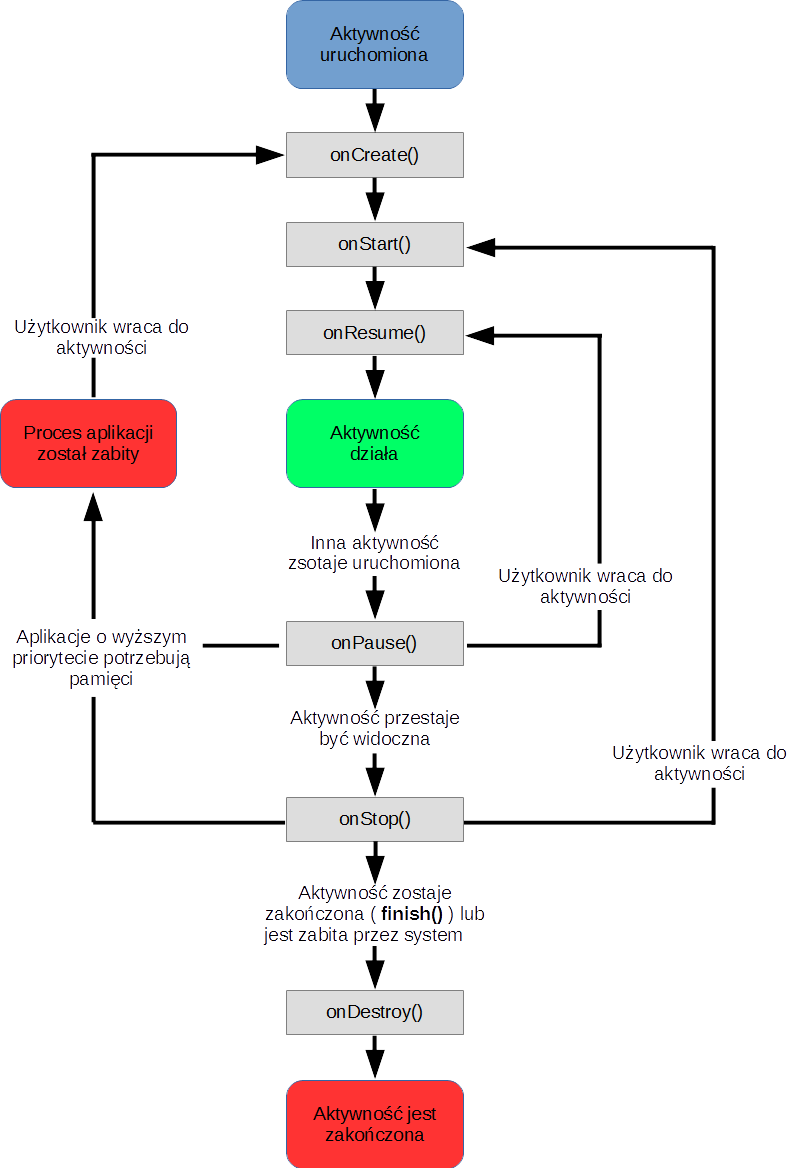
\includegraphics[width=10cm]{imgs/ch2_activity_lifecycle.png}
    \caption{Cykl życia \textit{Activity}\cite{website:android:aktywnosci}}
    \label{fig:sample_figure}
\end{figure} 


\item{Dostęp do baz danych i~do systemu plików}

Należy sprawdzić, czy operacje dostępowe przeprowadzane są poprawnie, a~jeżeli nie, to czy również poprawnie działa obsługa błędów. Można to testować na dwa sposoby: albo na niskim poziomie, izolując warstwę użytkownika, albo bezpośrednio z~aplikacji. Do testowania na niskim poziomie można wykorzystywać dostarczane przez framework Androida w~pakiecie \texttt{android.test.mock} \textit{zaślepki}\footnote{Zaślepka (stub) - szkieletowa albo specjalna implementacja modułu używana podczas produkcji lub testów innego modułu, który tę zaślepkę wywołuje albo jest w~inny sposób od niej zależny. Zaślepka zastępuje wywoływany moduł. [wg. IEEE 610]}

Według dokumentacji Android\cite{website:android:manual} możliwe są następujące opcje przechowywania danych:

- \textit{Shared Preferences}, czyli zachowywanie podstawowych danych w~parach klucz - wartość,

- pamięć wewnętrzna urządzenia - do zachowywania danych niepublicznych,

- zewnętrzna karta pamięci - do zachowywania danych publicznych,

- baza danych SQLite - do przechowywania danych w~prywatnej bazie danych,

- zasoby sieciowe - jako baza danych współdzielona pomiędzy urządzeniami.

Wszystkie te opcje korzystają ze wspólnego zestawu funkcji\footnote{Na przykład do obsługi plików używa się \textit{getFileDir(), getDir(), deleteFile()} itp.}, które tester powinien wziąć pod uwagę przy tworzeniu przypadków testowych.

\item{Fizyczną charakterystykę urządzenia}

Android został zaprojektowany do pracy na wielu różnych typach urządzeń, od telefonów do tabletów i~telewizorów. Deweloperzy muszą tolerować pewną zmienność zachowań projektowanych funkcji i~zapewnić elastyczny interfejs użytkownika, który dostosowuje się do różnych konfiguracji ekranu czy sieci.

Należy sprawdzić, czy aplikacja działa poprawnie na wszystkich urządzeniach, na których można ją uruchomić. To, że działa świetnie na smartfonie, nie znaczy że działa poprawnie na tablecie, a~to że działa na tablecie jednej firmy nie wyklucza awarii na tym samym urządzeniu wyprodukowanym przez kogoś innego. Elementy, które należy testować w~tym zakresie, to:

- możliwości sieciowe,

- rozdzielczość ekranu,

- gęstość ekranu,

- rozmiar ekranu,

- czułość sensorów,

- klawiaturę i~inne urządzenia wejściowe,

- lokalizację GPS,

- zewnętrzne karty pamięci.

Android framework dostarcza rozwiązań pozwalających dostosowywać pewne rzeczy automatycznie, ale nie zwalnia to projektantów przed wykonaniem zestawu niezbędnych testów również w~tym obszarze.

\end{itemize}

\section{Rodzaje testów}
Proces testowania może zostać wprowadzony na każdym etapie tworzenia aplikacji, w~zależności od wybranej strategii testu. Jednakże, jak już autor wspomniał w~podrozdziale \ref{czy_testowanie_potrzebne}, najlepiej jest rozpoczynać testowanie tak szybko jak to jest możliwe, w~możliwie najwcześniejszym stadium projektu. Nawet jeżeli nie wszystkie wymagania systemowe zostały uzgodnione, a~proces pisania oprogramowania się jeszcze nie rozpoczął. Już sam etap tworzenia dokumentacji i~wymagań, czy to na poziomie klienta, systemowym, czy softwarowym, powinien zostać poddany testowaniu. Pozwala to unikać błędów już na etapie wczesnego projektowania, a~które mogłyby wpływać na proces tworzenia przez długi czas.

Rozpoznaje się kilka poziomów testowania, w~zależności od modelu zarządzania projektem. Rozważając model V przedstawiony na schemacie \ref{fig:model_v}, wyróżnić możemy cztery główne interesujące z~punktu widzenia testowalności obszary:

\begin{itemize}
\item
testy jednostkowe (\textit{Unit tests})
\item
testy integracyjne
\item
testy systemowe
\item
testy akceptacyjne

\end{itemize}

\begin{figure}[!htb]
    \centering
    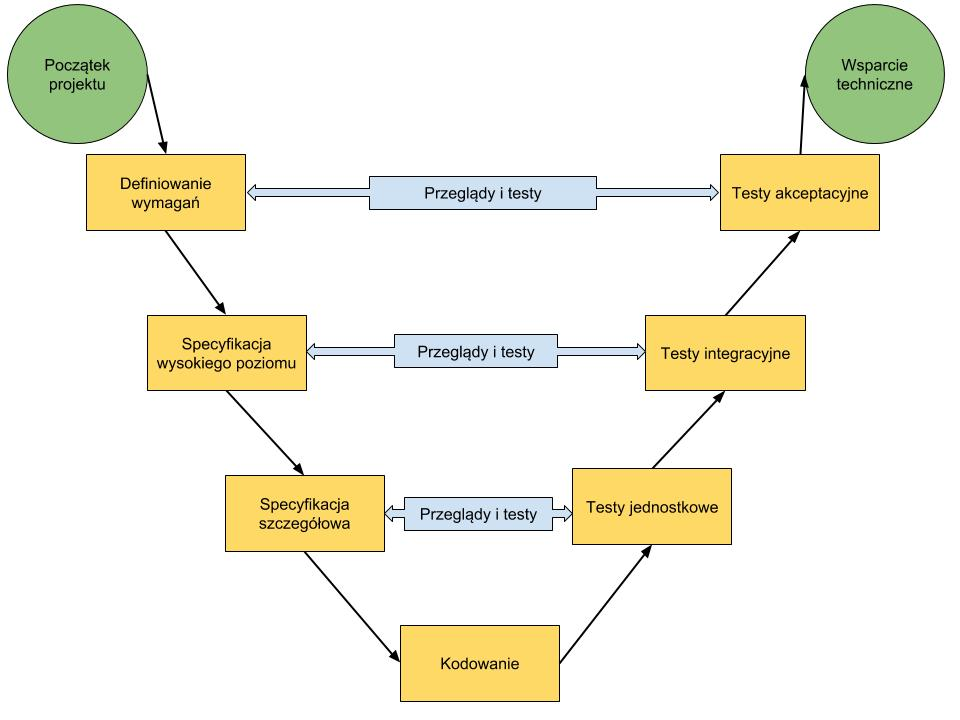
\includegraphics[width=10cm]{imgs/ch2_model_v_pl.jpg}
    \caption{Model V - najpopularniejszy model zarządzania projektem informatycznym (\textit{V\-model}) \cite{website:android:modelv}.}
    \label{fig:model_v}
\end{figure} 

\subsection{Testy jednostkowe (modułowe)}

Według \cite{bib:sylabus:foundation}, testy modułowe polegają na wyszukiwaniu błędów i~weryfikacji funkcjonalności oprogramowania (np. modułów, programów, obiektów, klas), które można testować oddzielnie. Testowanie może być wykonywane w~izolacji od reszty systemu, w~zależności od kontekstu cyklu rozwoju oprogramowania i~od samego systemu. Podczas testów można użyć zaślepek, sterowników testowych oraz symulatorów. 

Mogą one zawierać testy funkcjonalności oraz niektórych atrybutów niefunkcjonalnych, takich jak stopień wykorzystania zasobów (np. wycieków pamięci) lub odporności. Wlicza się w~nie również testy strukturalne - pokrycia linii kodu, decyzji lub gałęzi. Do projektowania przypadków testowych bardzo przydatna jest specyfikacja fumkcji. Wtedy jest możliwość zaprojektowania testów zanim zostanie napisany kod programu (tzw. "wytwarzanie sterowane testowaniem" - \textit{Test Driven Development}, opisane szerzej w~sekcji \ref{test_driven_development}). Testy modułowe zwykle wykonuje się mając dostęp do kodu źródłowego i~przy wsparciu środowiska rozwojowego (np. bibliotek do testów jednostkowych, narzędzi do debagowania). Testy jednostkowe w~praktyce zwykle angażują też programistę, który jest autorem kodu. Usterki są usuwane jak tylko zostaną wykryte, bez systemu formalnego nimi zarządzania nimi.

Najczęściej wykorzystywanym środowiskiem testowym dla Unit Testów pod Androidem jest \textit{JUnit}. To proste i~użyteczne narzędzie, pozwalające automatyzować testy jednostkowe, zostało zaprojektowane przez Ericha Gamma\footnote{Erich Gamma - szwajcarski informatyk, współautor książki "Wzorce projektowe: elementy oprogramowania obiektowego wielokrotnego użytku". Wspólnie z~Kentem Beckiem napisał narzędzie do tworzenia testów jednostkowych JUnit. Rozwijał także środowisko Eclipse.} i~Kenta Becka i~wydane na licencji \textit{open source}\cite{website:opensource}.

Głównie badaniem tego rodzaju testów autor zajmował się będzie w~części doświadczalnej pracy magisterskiej, w~rozdziale \ref{analiza_testow}.

\subsection{Testy integracyjne}

Testy integracyjne służą do sprawdzania interfejsów pomiędzy modułami, interakcji z~innymi częściami systemu (takimi jak system operacyjny, system plików i~sprzęt) oraz zależności pomiędzy systemami.

Wykonuje je się zwykle, jeżeli tylko jest możliwość przetestowania integracji gotowych już modułów, przetestowanych testami jednostkowymi. Pojęcie testowania integracyjnego można rozszerzyć również na testowanie integracji pomiędzy różnymi systemami, a~nawet produktami różnych producentów.\cite{bib:sylabus:foundation}

\subsection{Testy systemowe}

Testy systemowe zajmują się zachowaniem produktu lub systemu. Zakres takich testów powinien być jasno określony w~głównym planie testów oraz w~planach testów poszczególnych poziomów. Testy systemowe mogą zawierać testy oparte na ryzyku lub wymaganiach, procesie biznesowym, przypadkach użycia lub wysokopoziomowych opisach słownych i~modelach zachowania systemu, interakcji z~systemem operacyjnym i~zasobami systemowymi.

Dąży się do tego, aby środowisko testowe w~przypadku testów systemowych było maksymalnie zbliżone do środowiska docelowego, w~którym projektowana aplikacja ma działać. Optymalnie byłoby pokryć wszystkie możliwe konfiguracje sprzętowe, aczkolwiek z~wielu powodów, głównie finansowych, firmy skupiają się na najczęściej wykorzystywanych przez użytkownikach urządzeniach.\cite{bib:sylabus:foundation} 

\subsection{Testy akceptacyjne}

Celem testów akceptacyjnych jest nabranie zaufania do systemu, jego części lub pewnych atrybutów niefunkcjonalnych. Wyszukiwanie usterek nie jest głównym celem tego rodzaju testowania. Testy akceptacyjne mogą oceniać gotowość systemu do wdrożenia i~użycia, chociaż nie muszą być ostatnim poziomem testowania. Na przykład może po nich następować testowanie integracji systemów w~większej skali.

Odpowiedzialność za testy akceptacyjne, w~przeciwieństwie do testów opisanych w~poprzednich paragrafach, leży po stronie klientów. Zwykle testy akceptacyjne dzieli się na dwa etapy: testy \textit{alfa} oraz \textit{beta}. Testy \textit{alfa} przeprowadzane są przez przyszłych użytkowników w~siedzibie producenta, natomiast \textit{beta} - w~środowisku docelowym. w~praktyce producenci oprogramowania przekazują darmowe wersje swoich aplikacji o~ograniczonych możliwościach, oczekując w~zamian od użytkowników raportowania błędów lub propozycji usprawnień, bądź uzyskując to raportowanie automatycznie, kiedy aplikacja sama wysyła do producenta informację o~zaistniałych defektach.\cite{bib:sylabus:foundation}

\section{Zwinne podejście do testowania}
\subsection{Wytwarzanie sterowane testowaniem - \textit{Test Driven \newline Development}}
\label{test_driven_development}
Technika wytwarzania sterowanego zarządzaniem zyskuje coraz więcej popularności. Związane to jest pośrednio z~nowymi modelami zarządzania projektami informatycznymi opartymi na metodykach zwinnych, w~tym Agile\footnote{Agile software development – grupa metodyk wytwarzania oprogramowania opartego na programowaniu iteracyjno-przyrostowym, powstałe jako alternatywa do tradycyjnych metod typu \textit{waterfall\footnote{Iteracyjny model kaskadowy (ang. waterfall model) – jeden z~kilku rodzajów procesów tworzenia oprogramowania zdefiniowany w~inżynierii oprogramowania. Polega on na wykonywaniu podstawowych czynności jako odrębnych faz projektowych, w~porządku jeden po drugim. Każda czynność to kolejny schodek (kaskada). Jeśli któraś z~faz zwróci niesatysfakcjonujący produkt, należy się cofnąć wykonując kolejne iteracje aż do momentu kiedy otrzymano satysfakcjonujący produkt na końcu schodków. \textit{"Model kaskadowy", Wikipedia, 2014}}}. Najważniejszym założeniem metodyk zwinnych jest obserwacja, że wymagania odbiorcy (klienta) często ewoluują podczas trwania projektu. Oprogramowanie wytwarzane jest przy współpracy samozarządzalnych zespołów, których celem jest przeprowadzanie procesów wytwarzania oprogramowania. \textit{"Programowanie zwinne", Wikipedia, 2016}}. W~założeniu podejście takie pozwala:

\begin{itemize}
\item znaleźć więcej błędów na wcześniejszym etapie procesu developmentu;
\item świadomie zrobić zmiany wtedy, kiedy są potrzebne;
\item łatwo wykonać testy regresywne bazując na wcześniej napisanych procedurach;
\item przedłużyć żywotność kodu.
\end{itemize}

Jeżeli istnieją unit testy i~pokrywają znaczącą część kodu źródłowego, wtedy jasne jest, że więcej błędów zostanie znalezionych i~poprawionych. w~ten sam sposób przy podejściu \textit{Test Driven Development (TDD)} można wywnioskować, że skoro unit testy są już napisane, z~dużym prawdopodobieństwem pokrycie kodu będzie zadowalające. Co więcej, raz napisane testy można wykorzystywać do przeprowadzania testów regresywnych, aby się upewnić, czy zmiany w~naszym oprogramowaniu zgodne są z~założeniami i~wymaganiami systemu.

Testy jednostkowe w~podejściu TDD zapewniają, że jakość oprogramowania nie jest oparta na domysłach i~przekonaniu programistów, a~na rzetelnych raportach. Bez obaw można dokonywać modyfikacji takich, jak zmiana serwera baz danych, zmiana designu, interfejsu użytkownika, czy nawet API. Jeżeli wszystkie testy zostaną sprawdzone pozytywnie - oprogramowanie będzie działać nadal bezbłędnie.

Ponadto TDD zmusza developera, żeby napisał tylko tyle linijek kodu, ile jest niezbędne dla powstania i~działania danej fukcjonalności. Nie ma tu miejsca na wymyślanie własnych ścieżek i~innowacji. Należy trzymać się prostych rozwiązań tak mocno, jak to możliwe, a~co za tym idzie nie komplikować niepotrzebnie aplikacji.

Z powyższego można wnioskować, że podejście \textit{TDD} może znacznie pomóc w~zwiększeniu testowalności i~pielęgnowalności aplikacji. 

\subsection{Wytwarzanie sterowane zachowaniem - \textit{Behaviour Driven Development}}
\label{behaviour_driven_development}
BDD do kolejna technika testowania mająca swoje korzenie w~metodykach zwinnych. Wywodzi się bezpośrednio z~opisywanej wcześniej TDD, a~także  nawiązuje pośrednio do techniki \textit{Acceptance Test Driven Development} (ATDD), opisanej w~skrócie w~sekcji \ref{alternatywne_metody_testowania}.

BDD rozszerza TDD o~następujące elementy:
\begin{itemize}
\item
Wprowadza zasadę "pięciu pytań \textit{Dlaczego}" dla każdego proponowanego przypadku użycia (\textit{user story}). w~ten sposób łatwiej jest ustalić rzeczywisty cel biznesowy.

\item
Stosuje strategię myślenia "z zewnątrz do wewnątrz", czyli programowania tylko tego, co jest rzeczywiście potrzebne z~punktu widzenia biznesowego.

\item
Wprowadza jednoznaczny opis zachowania, tak aby z~tej samej dokumentacji lub notatki mogli korzystać zarówno programiści, jak i~testerzy i~eksperci systemowi.

\item
Ten sposób działania wprowadzany jest od najwyższego (wymagania użytkownika) aż do najniższego (wymagania funkcjonalne) poziomu abstrakcji.

\end{itemize}

Dokumentacja w~podejściu BDD oparta jest w~znacznej mierze na przypadkach użytkownika (\textit{user stories}). Oczywiście na niższych poziomach abstrakcji muszą one być odpowiednio uszczegółowione.

Główna różnica pomiędzy TDD a~BDD jest więc taka, że TDD odnosi się do testów, a~BDD do scenariuszy użycia, lub innych przypadków opisanych za pomocą charakterystycznych dla \textit{Behaviour Driven Development} form \textit{Given-When-Then\footnote{GWT - forma tworzenia specyfikacji na podstawie przykładów}} (GWT).

Wszystkie te elementy powinny doprowadzić do zwiększonej współpracy programistów, testerów oraz specjalistów i~ekspertów dziedzinowych. Zamiast terminu "testy jednostkowe", zwolennicy BDD wolą używać "specyfikacja zachowania klasy", a~zamiast "testy funkcjonalne" - "specyfikacja zachowania produktu".

Stosowanie techniki \textit{Behaviour Driven Development} nie wymaga żadnych specjalnych narzędzi ani języków programowania. Jest to podejście czysto koncepcyjne.\cite{website:agile:guide}

\subsection{Alternatywne techniki testowania}
\label{alternatywne_metody_testowania}
TDD i~BDD to nie jedyne strategie testowania, które można przyjąć zwiększając testowalność aplikacji androidowych. Warto wspomnieć również o~może nie tak popularnej, ale równie skutecznej strategii dotyczącej szczególnie testów akceptacyjnych, a~jest nią \textit{Acceptance Test-Driven Development} (ATDD). Jest to metodologia rozwoju opartego na komunikacji między klientami biznesowymi, programistami i~testerami. 

ATDD jest ściśle związane z~Test-Driven Development. Nacisk na współpracę z~wymaganiami klienckimi i~systemowymi jest tutaj zdecydowanie większy niż w~przypadku TDD, a~wykorzystywana jest przede wszystkim przy tworzeniu testów akceptacyjnych.

Analizując jeszcze głębiej metodyki zwinne, możemy doszukać się również podejść \textit{Example Driven Development} (EDD) oraz \textit{Story test-Driven Development} (SDD). Różnice między nimi a~\textit{TDD} są tak niewielkie, że autor pominie ich szczegółowy opis sygnalizując tylko, że zastosowanie takich taktyk testowania również może mieć wpływ na poprawienie testowalności aplikacji pod Androidem.  

%\section{Testowalność aplikacji androidowych}
%Z obserwacji autora wynika, że bardzo łatwo jest napisać zły i~nietestowalny kod dla Androida. Warto jednak pamiętać, że zastosowanie procesów z~metodologii wymienionych w~poprzednich podrozdziałach zdecydowanie może podnieść testowalność aplikacji pisanych dla tego systemu. Techniki te znacznie pomagają programistom i~testerom w~zrozumieniu potrzeb klienta.

%Ale czy zastosowanie metody \textit{TDD} lub \textit{BDD} jest wystarczające, aby podnieść testowalność aplikacji Android? Czy może potrzebna jest zmiana całej struktury aplikacji? Jak dzielić odpowiedzialność pomiędzy częściami oprogramowania? Jak rozwiązać problem zbyt dużego sprzężenia zarówno w~napisanym kodzie, jak i~pomiędzy kodem aplikacji i~frameworkiem androidowym \footnote{Sprzężenie (\textit{ang. coupling}) jest miarą jak bardzo obiekty, podsystemy lub systemy zależą od siebie nawzajem.}? Oraz najważniejsze pytanie: jak testować aplikacje dla Androida skutecznie?

%Na te pytania autor postara się odpowiedzieć w~dalszej części pracy.
%tutaj przykłady jak użyć poszczególnych konstrukcji
%Przykładowy rysunek \ref{fig:sample_figure}. Prztykładowa tabela %\ref{tab:sample_table}. Przykładowy odnośnik do bibliografi \cite{bib:kowalski_2015}. \textbf{Powodzenia!}


%\begin{figure}[!htb]
%    \centering
%    \includegraphics[width=10cm]{imgs/sample_figure.jpg}
%    \caption{Przykłady rysunek}
%    \label{fig:sample_figure}
%\end{figure} 

%\begin{table}[]
%\centering
%\caption{Przykładowa tabela}
%\label{tab:sample_table}
%\begin{tabular}{|l|l|}
%\hline
%\textbf{Nazwa} & \textbf{Wartość} \\ \hline
%Test           & 1.2              \\ \hline
%Kwiatek        & 5                \\ \hline
%\end{tabular}
%\end{table}